\documentclass{beamer}
%\mode<presentation>
\usepackage[utf8]{inputenc}
\usepackage[english]{babel}
\usetheme{CambridgeUS}
\usecolortheme{dolphin}
\usepackage{amsmath,amssymb,amsfonts, bm}
\usepackage{mathpazo}
\usepackage{graphicx,tabularx,epsfig}
\usepackage[compatibility=false]{caption}
\usepackage{subcaption}
\usepackage{rotating}


\setbeamertemplate{background}{\tikz[overlay,remember picture]\node[opacity=0.07]at (current page.center){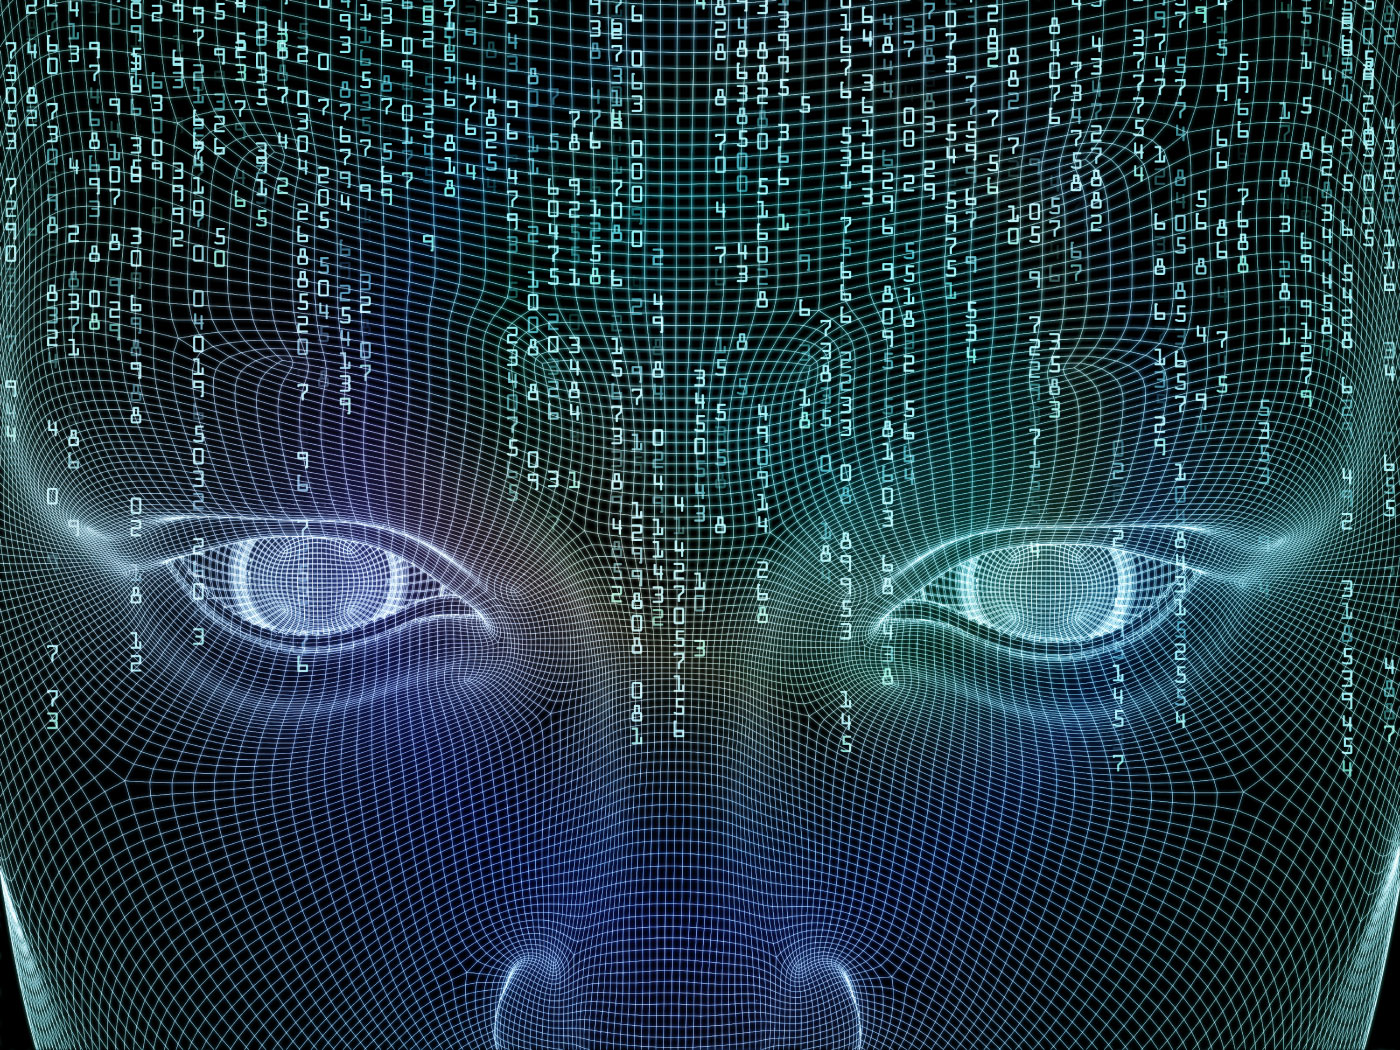
\includegraphics[width=\paperwidth]{pic/bkg}};}
\usepackage{tikz}

\DeclareGraphicsExtensions{.pdf,.png,.jpg,.svg}


\setbeamertemplate{itemize items}[square]
\setbeamertemplate{enumerate items}[square]

\definecolor{Red}{RGB}{190,0,0}
\definecolor{Blue}{RGB}{0,0,190}
\setbeamertemplate{headline}{}



\title[HBT]{Three particle Bose-Einstein correlation}
\author[Attila Bagoly]{Attila Bagoly\\ Eötvös Loránd University \vspace{0.5cm}}
\date[2016.10.20.]{2016.10.20}
\institute[ELTE]{
\large{Supervisor: Máté Csanád}
}

\begin{document}

\begin{frame}
  \titlepage
\end{frame}

\begin{frame}
\frametitle{Contents}
\tableofcontents
\end{frame}


\section{Introduction}
\begin{frame}
\frametitle{Introduction}
\begin{itemize}
\setlength{\itemsep}{12pt}
\item We want to obtain new information about sQGP by measuring 3 particle BE
\item Definition of correlation function:
\begin{equation}
C_3(\bm{k_1}, \bm{k_2}, \bm{k_3})=\frac{N_3(\bm{k_1}, \bm{k_2}, \bm{k_3})}{N_1(\bm{k_1})N_1(\bm{k_2})N_1(\bm{k_3})} \label{eq:e1}
\end{equation}
\item Where the particle number is defined by:
\begin{equation}
N_1(\bm{k})=\int S(\bm{x}, \bm{k})|\psi_1(\bm{x}, \bm{k})|^2 d^4x \label{eq:e2}
\end{equation}
\begin{align}
N_3(\bm{k_1}, \bm{k_2}, \bm{k_3})=\int S(\bm{x_1}, \bm{k_1})S(\bm{x_2}, \bm{k_2})S(\bm{x_3}, \bm{k_3})\nonumber\cdot\\\cdot|\psi_3(\bm{x_1},\bm{x_2},\bm{x_3}, \bm{k_1},\bm{k_2},\bm{k_3})|^2 d^4x_1d^4x_2d^4x_3\label{eq:e3}
\end{align}
\end{itemize}
\end{frame}

\begin{frame}
\frametitle{Introduction}
\begin{itemize}
\setlength{\itemsep}{12pt}
\item For free particles:
\begin{equation}
\psi(\bm{x}, \bm{k})\propto e^{-i\bm{x}\bm{k}}
\end{equation}
 $C_3$ can be expressed as function of $\bm{k_{ij}}=\bm{k_i}-\bm{k_j}$ and $\bm{K_{ij}}=\frac{1}{2}(\bm{k_i}+\bm{k_j})$
\item Same as in 2 particle analysis we expect: $\bm{k_{ij}}$ main kinematic variable, $\bm{K_{ij}}$ dependency smoother:
\begin{equation*}
\bm{K_{ij}} \rightarrow p_T=\sqrt{\bm{K_{12x}}^2+\bm{K_{12y}}^2+\bm{K_{13x}}^2+\bm{K_{13y}}^2+\bm{K_{23x}}^2+\bm{K_{23y}}^2}/3
\end{equation*}
\item So we want to measure $C_3(\bm{k_{12}}, \bm{k_{13}}, \bm{k_{23}})$ for different $p_T$ bins
\end{itemize}
\end{frame}

\begin{frame}
\frametitle{Introduction}
\begin{itemize}
\setlength{\itemsep}{12pt}
\item $C_3$ can be measured as various decomposition of components of relative momentum
\item We use side-out-longitudinal (Bertsch-Pratt) decomposition 
\item Coordinate system: LCMS (longitudinal co-moving system) of the three particle
\item Instead of $\bm{k_{ij}^{\mathrm{LCMS}}}$ we measure correlation as function of 
\begin{equation*}
k_{ij}=|\bm{k_{ij}^{\mathrm{LCMS3}}}|
\end{equation*}
\item Reason: in 2 particle analysis we have seen $C_2$ do not depend significantly on the orientation of $\bm{k}$
\end{itemize}
\end{frame}

\section{What and how we measure}
\begin{frame}
\frametitle{Details of measurement}
\begin{itemize}
\setlength{\itemsep}{22pt}
\item We use the so called event-mixing method to measure correlation
\item We take the momentum difference distributions of pion pairs within the triplet from same event: $A(k_{12}, k_{13}, k_{23})$
\item $A$ will contain effects as acceptance, kinematics, etc.
\item To transform this out: we create a background distribution ($B(k_{12}, k_{13}, k_{23})$) for triples which members are from different events
\end{itemize}
\end{frame}

\begin{frame}
\frametitle{Details of measurement}
\begin{itemize}
\setlength{\itemsep}{16pt}
\item The correlation:
\begin{equation}
C_3(k_{12}, k_{13}, k_{23})=\frac{A(k_{12}, k_{13}, k_{23})}{B(k_{12}, k_{13}, k_{23})}\frac{\int B(k_{12}, k_{13}, k_{23})dk_{12}dk_{13}dk_{23}}{\int A(k_{12}, k_{13}, k_{23})dk_{12}dk_{13}dk_{23}}
\end{equation}
\begin{figure}
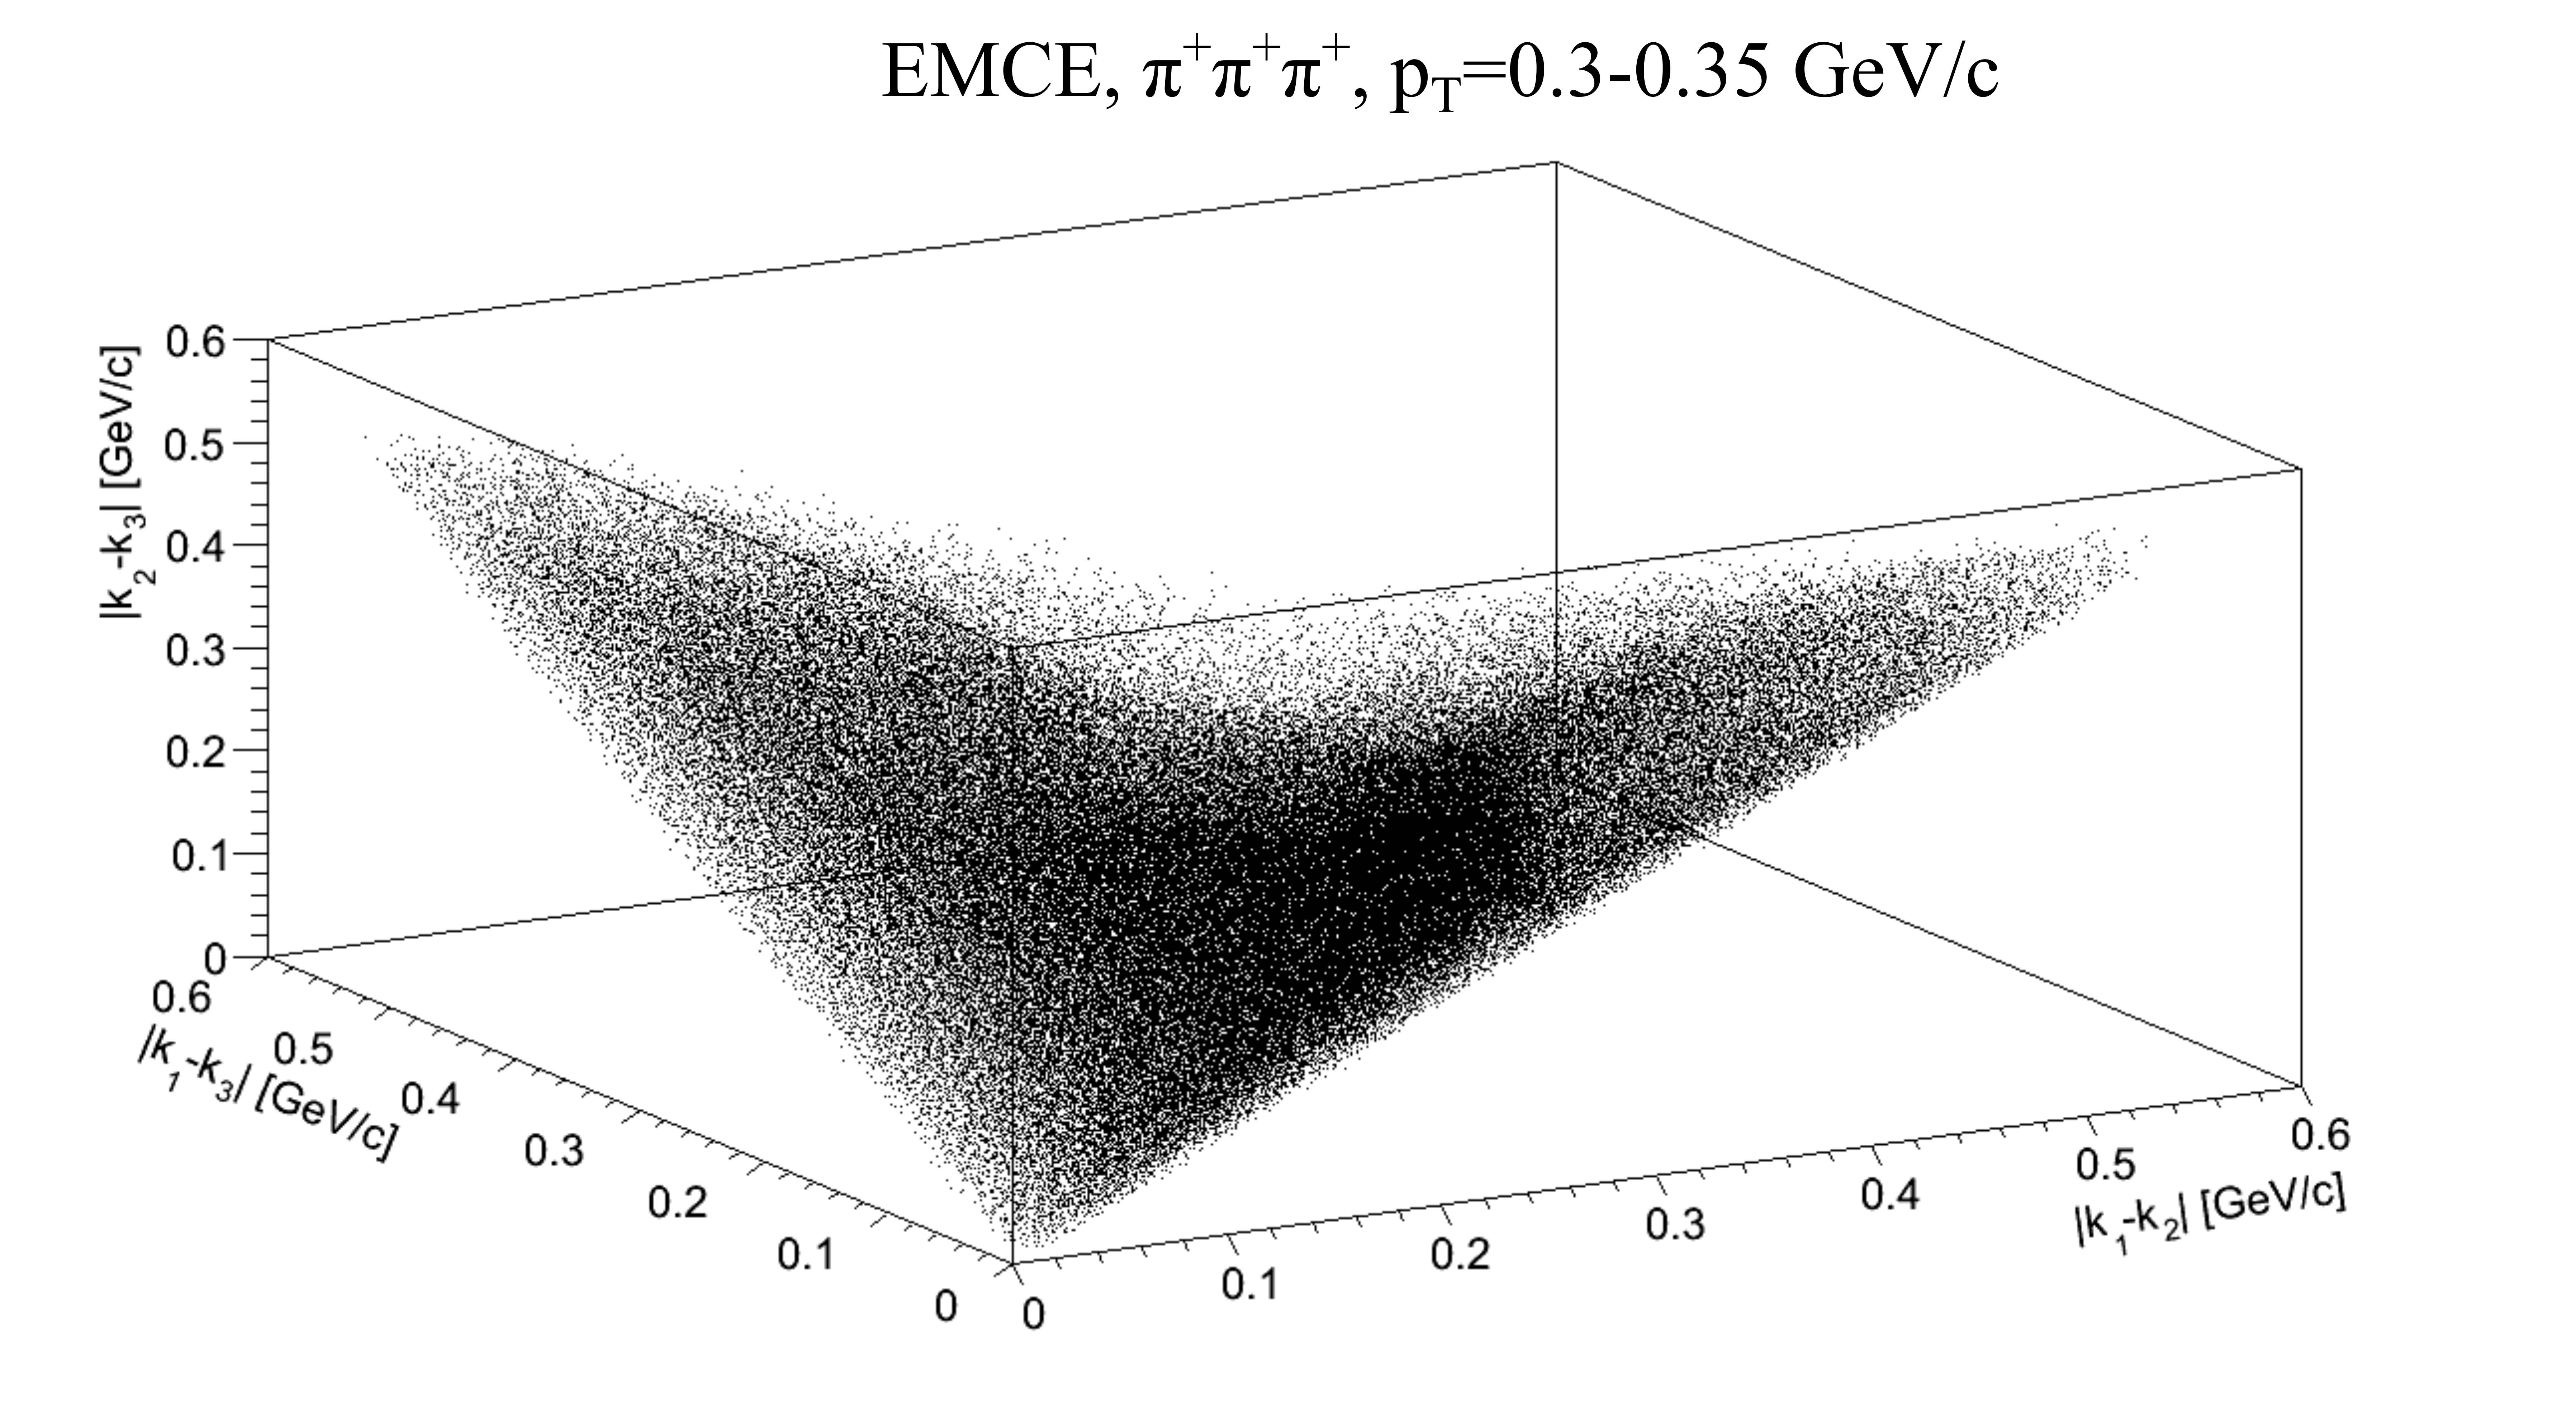
\includegraphics[scale=0.25]{pic/C1}
\end{figure}
\end{itemize}
\end{frame}

\begin{frame}
\frametitle{Details of measurement}
\begin{itemize}
\setlength{\itemsep}{16pt}
\item Changing order of particles within triplet $\rightarrow$ new bin in histogram
\item But this is not physics $\rightarrow$ we force: $k_{12}<k_{13}<k_{23}$ order
\begin{figure}
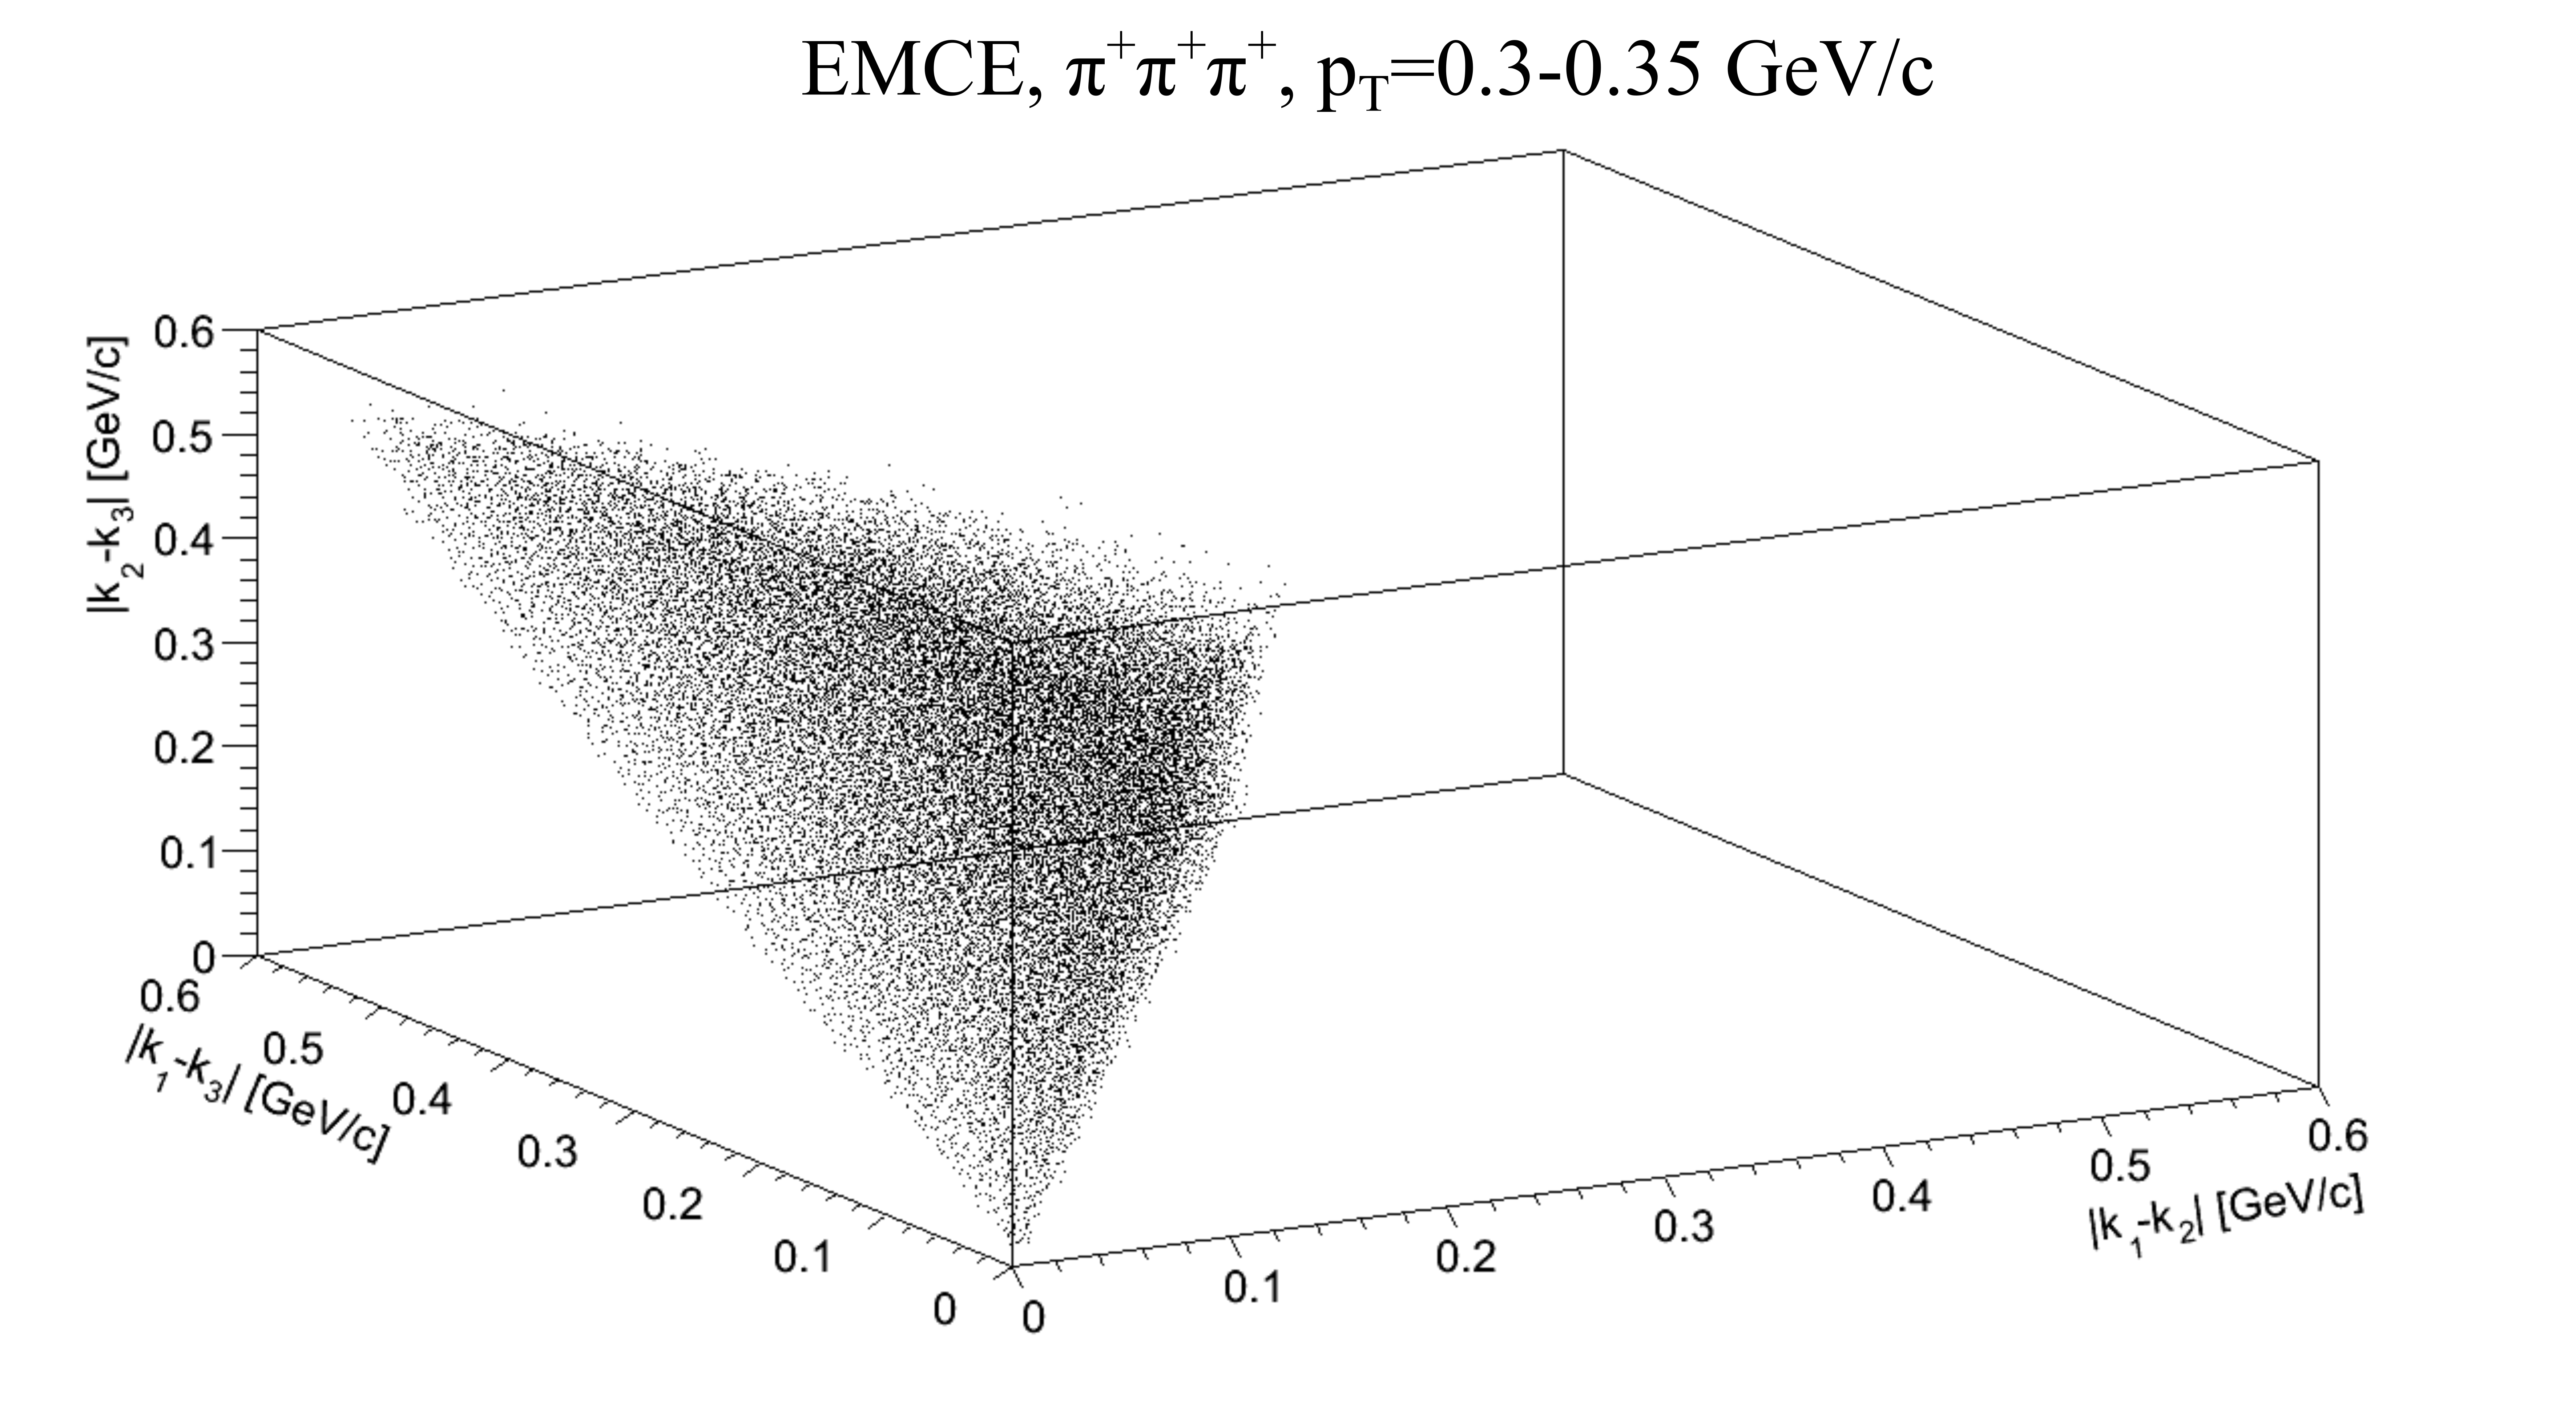
\includegraphics[scale=0.25]{pic/C2}
\end{figure}
\end{itemize}
\end{frame}

\section{Model}
\begin{frame}
\frametitle{Model without Coulomb correction}
\begin{itemize}
\setlength{\itemsep}{16pt}
\item Assumption for source: Levy-distribution
\begin{align}
\mathcal{L}(\alpha, R, r) = \frac{1}{(2\pi)^3}\int d^3 q e^{i\bm{q}\bm{r}}e^{-0.5|\bm{q} R|^\alpha}
\end{align}
\item The \ref{eq:e1}, \ref{eq:e2}, \ref{eq:e3} equations with free particle wave function:
\begin{align}
C_3^{(0)}(k_{12}, k_{13}, k_{23}) = 1+ Le^{-0.5(|2k_{12}R_C|^\alpha+|2k_{13}R_C|^\alpha+|2k_{23}R_C|^\alpha)}\nonumber\\
+f_C^2\bigg(e^{|2k_{12}R_C|^\alpha}+e^{|2k_{13}R_C|^\alpha}+e^{|2k_{23}R_C|^\alpha}\bigg)
\end{align}
\item $R_C$, $f_C$ same as in 2 particle case
\item We are looking for: $\lambda_3=L-3f_C^2$
\end{itemize}
\end{frame}

\begin{frame}
\frametitle{Coulomb correction}
\begin{itemize}
\setlength{\itemsep}{16pt}
\item Corrected model:
\begin{equation}
C_3(k_{12}, k_{13}, k_{23}) = C_3^{(0)}(k_{12}, k_{13}, k_{23})\cdot K_3(k_{12}, k_{13}, k_{23})
\end{equation}
\item We use Generalized Riverside method to handle the three particle Coulomb problem
\begin{equation}
K_3(k_{12}, k_{13}, k_{23}) = K_1(k_{12})K_1(k_{13})K_1(k_{23})
\end{equation}
\begin{figure}
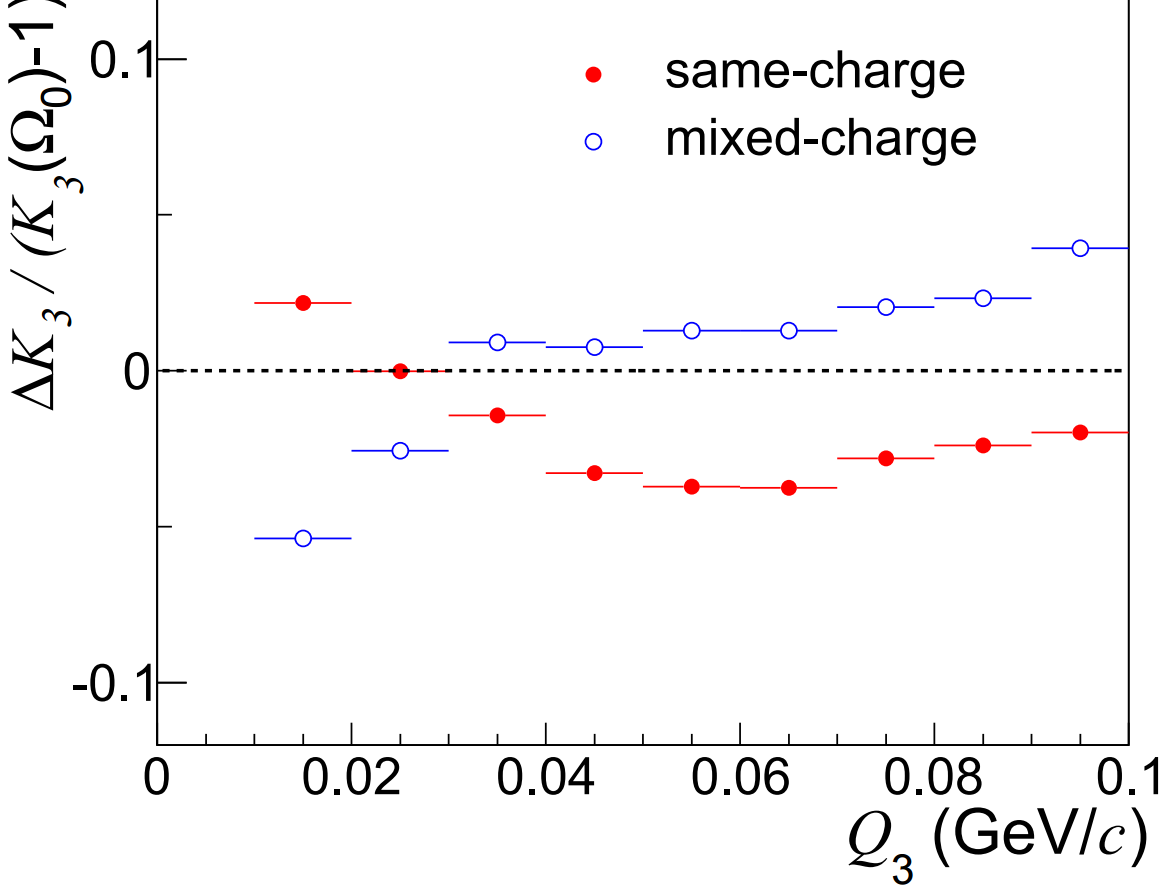
\includegraphics[scale=0.3]{pic/KKK}
\end{figure}
\end{itemize}
\end{frame}

\section{Analysis status}

\begin{frame}
\frametitle{Analysis status}
\begin{figure}
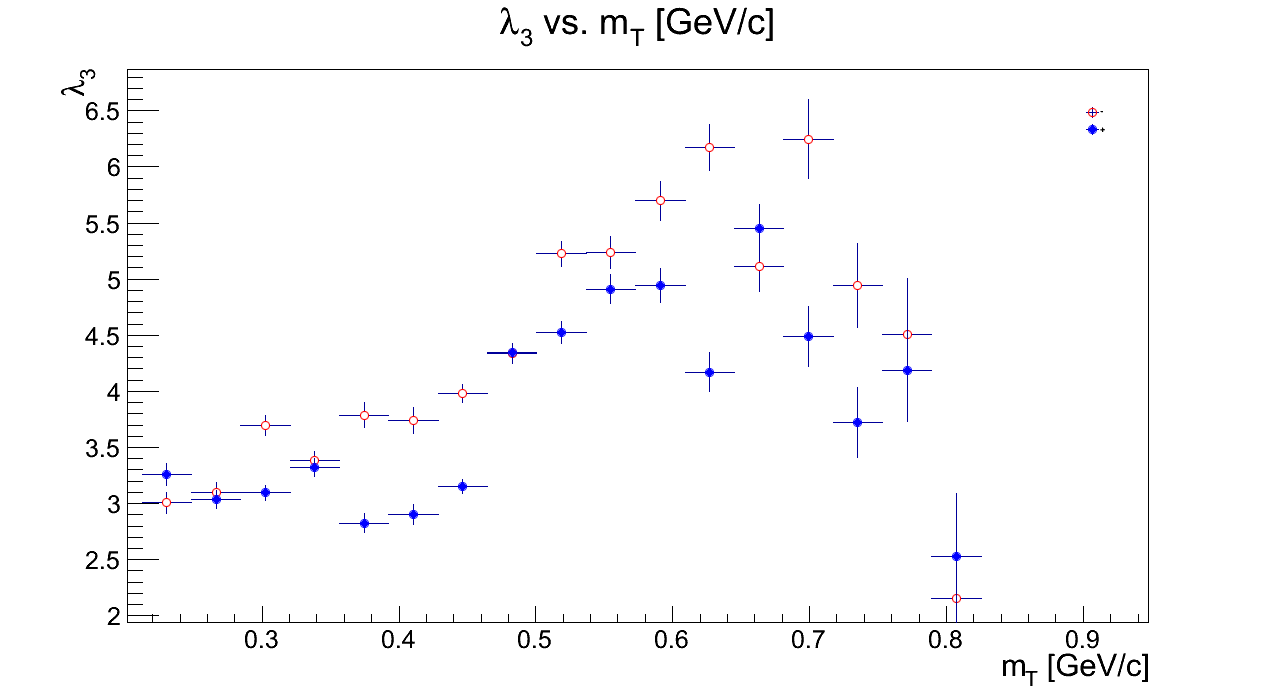
\includegraphics[scale=0.3]{pic/l3}
\end{figure}
\end{frame}

\begin{frame}
\frametitle{Analysis status}
\begin{figure}
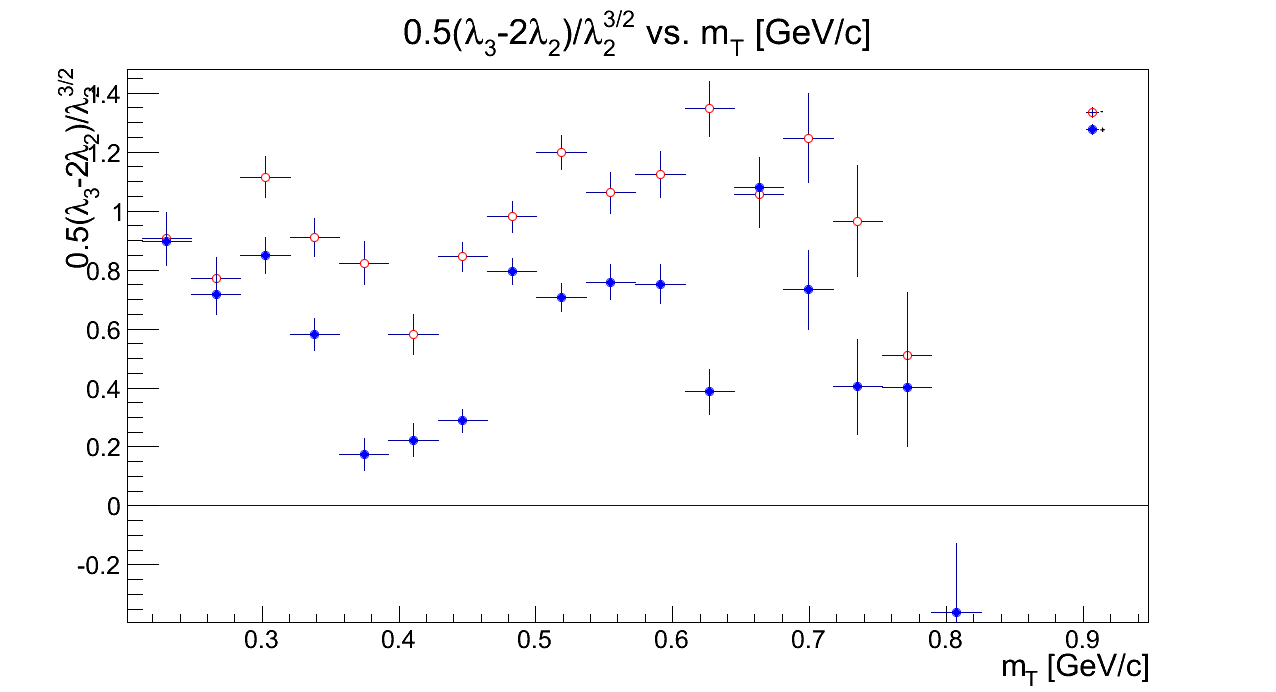
\includegraphics[scale=0.3]{pic/l4}
\end{figure}
\end{frame}





\end{document}

